\documentclass[11pt,border=5pt]{standalone}
\usepackage{fontspec}
\setmainfont{cmunrm.otf}[BoldFont=cmunbx.otf,ItalicFont=cmunti.otf,BoldItalicFont=cmunbi.otf]
\usepackage{amsmath}
\usepackage{unicode-math}
\setmathfont{NewCMMath-Regular.otf}
\usepackage{tikz}
\usetikzlibrary{arrows.meta,patterns,angles,quotes}
\begin{document}
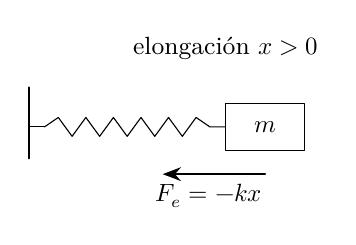
\begin{tikzpicture}[>=Stealth,font=\small,line cap=round,line join=round]
\draw[] (-3,0) -- (-2.8,0);
\draw (-2.800,0.000) -- (-2.625,0.120) -- (-2.450,-0.120) -- (-2.275,0.120) -- (-2.100,-0.120) -- (-1.925,0.120) -- (-1.750,-0.120) -- (-1.575,0.120) -- (-1.400,-0.120) -- (-1.225,0.120) -- (-1.050,-0.120) -- (-0.875,0.120) -- (-0.700,0.000) -- (-0.500,0.000);
\draw[fill=white] (-0.5,-0.3) rectangle (0.5,0.3);
\node at (0,0) {$m$};
\draw[thick] (-3,-0.4) -- (-3,0.5);
\draw[->,thick] (0,-0.6) -- (-1.3,-0.6) node[pos=0.55,below] {$F_e=-kx$};
\node at (-0.5,1) {elongación $x>0$};

\end{tikzpicture}
\end{document}
